\documentclass[journal,12pt,twocolumn]{IEEEtran}

\usepackage{setspace}
\usepackage{gensymb}

\singlespacing


\usepackage[cmex10]{amsmath}

\usepackage{amsthm}

\usepackage{mathrsfs}
\usepackage{txfonts}
\usepackage{stfloats}
\usepackage{bm}
\usepackage{cite}
\usepackage{cases}
\usepackage{subfig}

\usepackage{longtable}
\usepackage{multirow}

\usepackage{enumitem}
\usepackage{mathtools}
\usepackage{steinmetz}
\usepackage{tikz}
\usepackage{circuitikz}
\usepackage{verbatim}
\usepackage{tfrupee}
\usepackage[breaklinks=true]{hyperref}
\usepackage{graphicx}
\usepackage{tkz-euclide}

\usetikzlibrary{calc,math}
\usepackage{listings}
    \usepackage{color}                                            %%
    \usepackage{array}                                            %%
    \usepackage{longtable}                                        %%
    \usepackage{calc}                                             %%
    \usepackage{multirow}                                         %%
    \usepackage{hhline}                                           %%
    \usepackage{ifthen}                                           %%
    \usepackage{lscape}     
\usepackage{multicol}
\usepackage{chngcntr}

\DeclareMathOperator*{\Res}{Res}

\renewcommand\thesection{\arabic{section}}
\renewcommand\thesubsection{\thesection.\arabic{subsection}}
\renewcommand\thesubsubsection{\thesubsection.\arabic{subsubsection}}

\renewcommand\thesectiondis{\arabic{section}}
\renewcommand\thesubsectiondis{\thesectiondis.\arabic{subsection}}
\renewcommand\thesubsubsectiondis{\thesubsectiondis.\arabic{subsubsection}}


\hyphenation{op-tical net-works semi-conduc-tor}
\def\inputGnumericTable{}                                 %%

\lstset{
%language=C,
frame=single, 
breaklines=true,
columns=fullflexible
}
\begin{document}


\newtheorem{theorem}{Theorem}[section]
\newtheorem{problem}{Problem}
\newtheorem{proposition}{Proposition}[section]
\newtheorem{lemma}{Lemma}[section]
\newtheorem{corollary}[theorem]{Corollary}
\newtheorem{example}{Example}[section]
\newtheorem{definition}[problem]{Definition}

\newcommand{\BEQA}{\begin{eqnarray}}
\newcommand{\EEQA}{\end{eqnarray}}
\newcommand{\define}{\stackrel{\triangle}{=}}
\bibliographystyle{IEEEtran}
\providecommand{\mbf}{\mathbf}
\providecommand{\pr}[1]{\ensuremath{\Pr\left(#1\right)}}
\providecommand{\qfunc}[1]{\ensuremath{Q\left(#1\right)}}
\providecommand{\sbrak}[1]{\ensuremath{{}\left[#1\right]}}
\providecommand{\lsbrak}[1]{\ensuremath{{}\left[#1\right.}}
\providecommand{\rsbrak}[1]{\ensuremath{{}\left.#1\right]}}
\providecommand{\brak}[1]{\ensuremath{\left(#1\right)}}
\providecommand{\lbrak}[1]{\ensuremath{\left(#1\right.}}
\providecommand{\rbrak}[1]{\ensuremath{\left.#1\right)}}
\providecommand{\cbrak}[1]{\ensuremath{\left\{#1\right\}}}
\providecommand{\lcbrak}[1]{\ensuremath{\left\{#1\right.}}
\providecommand{\rcbrak}[1]{\ensuremath{\left.#1\right\}}}
\theoremstyle{remark}
\newtheorem{rem}{Remark}
\newcommand{\sgn}{\mathop{\mathrm{sgn}}}
\providecommand{\abs}[1]{\vert#1\vert}
\providecommand{\res}[1]{\Res\displaylimits_{#1}} 
\providecommand{\norm}[1]{\Vert#1\rVert}
%\providecommand{\norm}[1]{\lVert#1\rVert}
\providecommand{\mtx}[1]{\mathbf{#1}}
\providecommand{\mean}[1]{E[ #1 ]}
\providecommand{\fourier}{\overset{\mathcal{F}}{ \rightleftharpoons}}
%\providecommand{\hilbert}{\overset{\mathcal{H}}{ \rightleftharpoons}}
\providecommand{\system}{\overset{\mathcal{H}}{ \longleftrightarrow}}
	%\newcommand{\solution}[2]{\textbf{Solution:}{#1}}
\newcommand{\solution}{\noindent \textbf{Solution: }}
\newcommand{\cosec}{\,\text{cosec}\,}
\providecommand{\dec}[2]{\ensuremath{\overset{#1}{\underset{#2}{\gtrless}}}}
\newcommand{\myvec}[1]{\ensuremath{\begin{pmatrix}#1\end{pmatrix}}}
\newcommand{\mydet}[1]{\ensuremath{\begin{vmatrix}#1\end{vmatrix}}}
\numberwithin{equation}{subsection}
\makeatletter
\@addtoreset{figure}{problem}
\makeatother
\let\StandardTheFigure\thefigure
\let\vec\mathbf
\renewcommand{\thefigure}{\theproblem}
\def\putbox#1#2#3{\makebox[0in][l]{\makebox[#1][l]{}\raisebox{\baselineskip}[0in][0in]{\raisebox{#2}[0in][0in]{#3}}}}
     \def\rightbox#1{\makebox[0in][r]{#1}}
     \def\centbox#1{\makebox[0in]{#1}}
     \def\topbox#1{\raisebox{-\baselineskip}[0in][0in]{#1}}
     \def\midbox#1{\raisebox{-0.5\baselineskip}[0in][0in]{#1}}
\vspace{3cm}
\title{Assignment-6}
\author{Satya Sangram Mishra}
\maketitle
\newpage
\bigskip
\renewcommand{\thefigure}{\theenumi}
\renewcommand{\thetable}{\theenumi}
Download all python codes from 
\begin{lstlisting}
https://github.com/satyasm45/Summer-Internship/tree/main/Assignment-6/Codes
\end{lstlisting}
%
and latex-tikz codes from 
%
\begin{lstlisting}
https://github.com/satyasm45/Summer-Internship/tree/main/Assignment-6
\end{lstlisting}
%
\section{Question No. 2.41}
Find the equation of all lines having slope 2 and being tangent to the curve $y+\frac{2}{x-3}=0$
%
\section{Explanation}
The equation of curve:
\begin{align}
  y+\frac{2}{x-3}=0  \\
  xy-3y+2=0\label{eq:giveneq}
\end{align}
Comparing with the standard equation :
\begin{align}
\vec{x}^T\vec{V}\vec{x}+2\vec{u}^T\vec{x}+f=0\\
\vec{V}=\myvec{0&\frac{1}{2}\\\frac{1}{2}&0},\vec{u}=\myvec{0\\-\frac{3}{2}},f=2\\
\vec{V}^{-1}=\myvec{0&2\\2&0}
\end{align}
$\because$
\begin{align}
    \abs{\vec{V}} &= \frac{-1}{4}
    \\
    \implies \abs{\vec{V}} &< 0
\end{align}
$\therefore$ \eqref{eq:giveneq} represents a hyperbola .
\\
Now,the characteristic equation of $\vec{V}$ is 
\begin{align}
    \abs{\vec{V} - \lambda\vec{I}} = \mydet{-\lambda & \frac{1}{2} \\ \frac{1}{2} & -\lambda} &= 0
    \\
    \implies \lambda^2 - \frac{1}{4} &= 0
\end{align}
$\therefore$ Eigen values are 
\begin{align}
    \lambda_1 = \frac{1}{2} , \lambda_2 = \frac{-1}{2}
\end{align}
Eigen vector $\vec{p}$ is 
\begin{align}
    \vec{V}\vec{p} &= \lambda\vec{p}
    \\
    \implies (\vec{V} - \lambda\vec{I})\vec{p} &= 0
\end{align}
Eigen vector $\vec{p}_1$ corressponding to $\lambda_1$ can be obtained as
\begin{align}
    (\vec{V} - \lambda_1\vec{I}) &= \myvec{\frac{-1}{2} & \frac{1}{2} \\ \frac{1}{2} & \frac{-1}{2}}\xleftrightarrow[R_1 \leftarrow -2R_1]{R_2 = R_1 + R_2}\myvec{1 & -1 \\ 0 & 0}
    \\
    \implies \vec{p_1} &= \frac{1}{\sqrt{2}}\myvec{1 \\ 1}
\end{align}
Similarly,
\begin{align}
    \vec{p_2} &= \frac{1}{\sqrt{2}}\myvec{-1 \\ 1}
\end{align}
$\therefore$
\begin{align}
    \vec{P} &= \myvec{\vec{p_1} & \vec{p_2}} = \frac{1}{\sqrt{2}}\myvec{1 & -1 \\ 1 & 1}
    \\
    \vec{D} &= \myvec{\lambda_1 & 0 \\ 0 & \lambda_2} = \myvec{\frac{1}{2} & 0 \\ 0 & \frac{-1}{2}}
\end{align}
Now,
\begin{align}
    \vec{c} &= -\vec{V}^{-1}\vec{u} 
    \\
    &= -\myvec{0 & 2 \\2 & 0}\myvec{0 \\ \frac{-3}{2}}
    \\
    &= \myvec{3 \\ 0}
\end{align}
\begin{align}
\vec{u}^T\vec{V}^{-1}\vec{u} - f<0
\end{align}
So axes need to be swapped.
\begin{align}
    \sqrt{\frac{ \vec{u}^T\vec{V}^{-1}\vec{u} - f}{\lambda_2}} &= 2
    \\
    \sqrt{ \frac{f- \vec{u}^T\vec{V}^{-1}\vec{u}}{\lambda_1}} &= 2
\end{align}
$\therefore$ Equation of standard hyperbola can be expressed as 
\begin{align}
    \frac{y^2}{4} - \frac{x^2}{4} &= 1
\end{align}
The direction and normal vectors of tangent with slope 2:
\begin{align}
    \vec{m}=\myvec{1\\2},\vec{n}=\myvec{-2\\1}
\end{align}
From conics table in manual:
\begin{align}
\kappa = \pm \sqrt{\frac{\vec{u}^T\vec{V}^{-1}\vec{u}-f}{\vec{n}^T\vec{V}^{-1}\vec{n}}} = \pm \sqrt{\frac{1}{4}} = \pm \frac{1}{2}
\end{align}
and the desired points of contact are 
\begin{align}
\vec{q}=\vec{V}^{-1}(\kappa\vec{n}-\vec{u})\\
\vec{q}_1=\myvec{4\\-2}\label{eq:9}\\
\vec{q}_2=\myvec{2\\2}\label{eq:10}
\end{align}
The equation of tangents are given by:
\begin{align}
    \vec{n}^T\vec{x}=\vec{n}^T\vec{q}=c\\
    \myvec{-2&1}\vec{x}=\myvec{-2&1}\myvec{4\\-2}=-10\\
    \myvec{-2&1}\vec{x}=\myvec{-2&1}\myvec{2\\2}=-2
\end{align}

\numberwithin{figure}{section}
\begin{figure}[!ht]
\centering
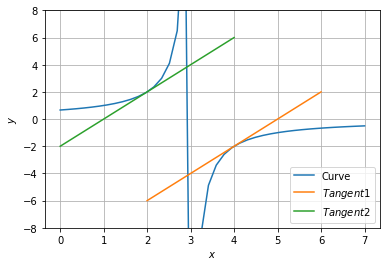
\includegraphics[width=\columnwidth]{figure6}
\caption{The tangents to the curve with slope 2 }
\label{fig:tangents}	
\end{figure}
\end{document}
